\section{Proofs from \cref{sec:probabilistic}}
\label{app:probabilistic}

In all of the following lemmas, we assume that $\eps_\eta \le \eps_{1/2}^2$ and $12\eps_{1/1}\leq \eps_{1/2}$.

\begin{figure}[htb]\centering
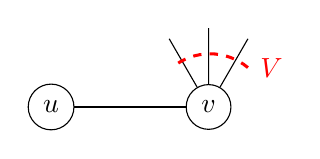
\begin{tikzpicture}
\node [draw,circle] at (0,0) (u) {$u$};
\node [draw,circle] at (2,0) (v) {$v$} edge node [below] {$\bbe$} (u);
\draw (v) -- +(60:1) (v) -- + (90:1) (v) -- +(120:1);
\draw [color=red,dashed,line width=1.1pt](2.5,0.5) arc (50:130:0.75);
\node [color=red] at (2.8,0.5) () {$V$};
\end{tikzpicture}
\caption{Setting of \cref{lem:x_e<=1/2-eps1}}
\label{fig:x_e<=1/2-eps1}
\end{figure}

\lemxesmallhalfeps*
\begin{proof}
Let $A,B,C$ be the \hyperlink{tar:degreepartition}{degree partitioning} of  $\delta(u)$.
Let $V:= \delta(v)_{-\bbe}$ (see \cref{fig:x_e<=1/2-eps1}).
Condition $u,v$ be trees, $\bbe$ and $C$ to 0, let $\nu$ be the resulting measure. This happens with probability at least  $0.5$ and increases marginals in $A_{-\bbe},B_{-\bbe}, V$ by at most $x_\bbe+2\eps_{1/1}+\eps_{\eta}\leq x_\bbe+2.1\eps_{1/1}$ and by tree conditioning decreases marginals by at most $2\eps_{\eta}$.  
%This conditioning increases marginals in $A, B$ and $D$ by at most $q$.
After conditioning, we have
\begin{align*}
&\EE{\nu}{A_T} \in x(A)-x_{\bbe(A)}+[-2\eps_\eta, x_\bbe+2.1\eps_{1/1}] %x(A [1/2 + \eps_{1/2}-\eps_{1/1}-2\eps_{\eta}, 1.5-\eps_{1/2}+2\eps_{1/1}+2\eps_{\eta}]
 \subset [0.5, 1.5], \text{ similarly }\EE{\nu}{B_T}\subset [0.5,1.5]\\
&\EE{\nu}{V_T} \in  x(\delta(v))-x_\bbe+ [-2\eps_\eta, x_\bbe+2.1\eps_{1/1}]\subset [1.5,2.01] %[2- (1/2 - \eps_1) - \eps_2, 2+ 2\eps _2] 
\\
&\EE{\nu}{B_T+V_T} \in x(B)+x(\delta(v))-x_\bbe - x_{\bbe(B)} + [-2\eps_\eta, x_\bbe+2.1\eps_{1/1}] 
%[2+ 2(\eps_{1/2} - \eps_{1/1}), ~3 + 2\eps_{1/1} ]
\subset [2+1.8\eps_{1/2}, 3.01],\\ % 1-\eps2 -(1/2-eps1) + 2- (1/2-\eps1) -eps2,     2+ \eps_2 (D) +  1+ 2 \eps_2 (A) + \eps 2 (C) 
&\EE{\nu}{A_T+B_T}\in x(A)+x(B)-x_{e(A)}-x_{\bbe(B)} + [-2\eps_\eta, x_\bbe+2.1\eps_{1/1}]\subset %[3/2-2\eps_{1/1} + \eps_{1/2},~ 2+2\eps_{1/1}]\subset 
[1.5, 2.01],\\
% 2-2\eps_2 - (1/2 - \eps_1) lb.
& \EE{\nu}{A_T+B_T+V_T} \in x(A)+x(B)+x(\delta(v))-x_\bbe-x_{e(A)}-x_{\bbe(B)}+ [-2\eps_\eta, x_\bbe+2.1\eps_{1/1}] \\ 
&\quad \quad \quad \quad \subset %[3+ 2\eps_{1/2} -3\eps_{1/1}, ~4 + 3\eps_{1/1}]\subset 
[3+1.75\eps_{1/2},4.01].  % 2 -2 eps2 (A+B) +  2- 2(1/2 - eps1)(xy) - eps2 (C) = 3 - 3 eps2 + 2 eps1 (lb),  2+ eps2 (D)  + 2 + eps2 (A,B) + eps2 (C)T
\end{align*}
where we used $\eps_{1/2}\leq 0.001$ and $12\eps_{1/1}<\eps_{1/2}$ and $x_{e(A)},x_{\bbe(B)},x_{e(A)}+x_{\bbe(B)}\leq x_\bbe\leq 1/2-\eps_{1/2}$.
It immediately follows from \cref{lem:427gen} that $\PP{\nu}{A_T=B_T=1,V_T=2}$ is at least a constant. In the rest of the proof, we do a more refined analysis. 
Using $A_T+B_T\geq 1, V_T\geq 1$,
\begin{align*}
&\PP{\nu}{A_T+B_T+V_T=4}\geq 	(1.75\eps_{1/2})e^{-1.75\eps_{1/2}} \geq 1.7\eps_{1/2}, \tag{\cref{thm:rayleigh_expectconstprob}} \\
&\PP{\nu}{A_T+B_T\geq 2},\PP{\nu}{V_T\geq 2} \geq 0.39, \tag{\cref{lem:SR>=}} \\
&\PP{\nu}{A_T+B_T\leq 2},\PP{\nu}{V_T\leq 2} \geq 0.5, \tag{Markov, $A_T+B_T\geq 1, V_T\geq 1$ under $\nu$} \\
&\PP{\nu}{A_T\leq 1}\geq 0.25, \PP{\nu}{B_T+V_T\leq 3} \geq 0.33. \tag{Markov's Inequality and $V_T\geq 1$ under $\nu$}\\
&\PP{\nu}{A_T\geq 1}\geq 0.39, \PP{\nu}{B_T+V_T\geq 3}\geq 1.75\eps_{1/2}, \tag{\cref{lem:SR>=}}
\end{align*}

It follows by \cref{lem:SRA=nA} (with $\eps=0.195, p_m\geq 1-2\eps\geq 0.6$) that 
$$\PP{\nu}{V_T=2 | A_T+B_T+V_T=4} \geq 0.13.$$
Note that since $V_T\geq 1, A_T+B_T\geq 1$ with probability 1, we apply \cref{lem:SRA=nA} to $V_T-1, A_T+B_T-1$.

Furthermore, by \cref{lem:updowntruncation}, $\PP{\nu}{A_T\geq 1 | A_T+B_T+V_T=4} \geq 0.128$, $\PP{\nu}{A_T\leq 1 | A_T+B_T+V_T=4} \geq 0.43\eps_{1/2}$. The same holds for $B_T$. Therefore, by \cref{lem:SRA=nA} (with $\eps=0.055\eps_{1/2}$), using that $\eps_{1/2}<0.001$,
$$\PP{\nu}{A_T=1 | A_T+B_T=2, V_T=2} \geq 0.05\eps_{1/2}.$$
Putting these together we have
\begin{align*} \P{e\text{ 2-1-1 happy}} &\geq 0.5 \PP{\nu}{A_T=B_T=1,V_T=2} \\
&= 0.5\PP{\nu}{A_T+B_T+V_T=4}\PP{\nu}{V_T=2|A_T+B_T+V_T=4}\\
&\quad \quad \cdot \PP{\nu}{A_T=1| V_T=2,A_T+B_T=2}\\
&\geq 0.5 (1.7\eps_{1/2})(0.13)(0.05\eps_{1/2}) \geq  0.005\eps_{1/2}^2
\end{align*}
as desired.
\end{proof}


\xemoreepshalf*
\begin{proof}
Let $A,B,C$ be the \hyperlink{tar:degreepartition}{degree partitioning} of the edges in $\delta(u)$, $V=\delta_{-\bbe}(v)$.
Condition $u, v$ be trees, $C_T=0$ and $u \cup v$ to be a tree (in order). This happens with probability at least $\frac12+\eps_{1/2}-3\eps_\eta-2\eps_{1/1}\geq 0.5$. Let $\nu$ be the resulting measure restricted to edges in $A,B,V$. 
Note that $\nu$ on edges in $A,B,V$ is SR.
This is because $\nu$ is a product of two strongly Rayleigh distribution on the following two disjoint set of edges (i) the edges between $u,v$ and (ii) the edges in $A_{-\bbe},B_{-\bbe},V$.

Furthermore, observe that under $\nu$, every set of edges in $A_{-\bbe},B_{-\bbe},V$ increases by at most $2\eps_{1/1}+\eps_\eta<0.2\eps_{1/2}$ (using $12\eps_{1/1}\leq \eps_{1/2}$), and decreases by at most $1-x_\bbe+2\eps_{\eta}$.  Therefore,
\begin{align*}
&\EE{\nu}{A_T} \in x(A)+[-(1-x_\bbe)-2\eps_{\eta},1-x_\bbe+0.2\eps_{1/2}]\subset   [0.5,1.5], \text{ similarly, }\EE{\nu}{B_T} \in [0.5,1.5]\\
& \EE{\nu}{V_T} \in x(\delta(v))-x_\bbe+ [-(1-x_\bbe)-2\eps_{\eta},0.2\eps_{1/2}] \subset [ 0.995 , 1.5].\\
&\EE{\nu}{A_T+B_T} \in x(A)+x(B)+1-x_{e(A)}-x_{\bbe(B)}+ [-(1-x_\bbe)-2\eps_{\eta},0.2\eps_{1/2}] \subset [1.995, 2.5],  \\
&\EE{\nu}{B_T+V_T}\in x(B)+x(\delta(v))-x_\bbe+ [-(1-x_\bbe)-2\eps_{\eta}, 1-x_\bbe+0.2\eps_{1/2}]\subset [1.99, 3-1.75\eps_{1/2}].\\
&\EE{\nu}{A_T+B_T+V_T} \in x(A)+x(B)+x(\delta(v))+1-x_\bbe-x_{e(A)}-x_{\bbe(B)}+[-(1-x_\bbe)-2\eps_{\eta},0.2\eps_{1/2}] \\
&\quad \quad \quad \quad \subset [2.99, 4-1.75\eps_{1/2}].
\end{align*}
where in the upper bound on $\EE{\nu}{A_T}$, $\EE{\nu}{B_T}$, $\EE{\nu}{B_T+V_T}$ we used that the marginals of edges in the bundle $\bbe$ can only increase by $1-x_\bbe$ (in total) when conditioning $u\cup v$ to be a tree.
So, 
\begin{align*} 
&\PP{\nu}{A_T+B_T+V_T=3} \geq \eps_{1/2}, \tag{By \cref{thm:hoeffding}}\\
% worst case: 4 Bernoullies with prob. $1-\frac{1.75}{4}\eps_{1/2}$}\\ 	
&\PP{\nu}{A_T+B_T\geq 2}\geq 0.63, \PP{\nu}{V_T\geq 1} \geq 0.63\tag{\cref{lem:SR>=}, $A_T+B_T\geq 1$}\\
&\PP{\nu}{A_T+B_T\leq 2}\geq 0.25, \PP{\nu}{V_T\leq 1}\geq 0.25, \tag{Markov Inequality, $A_T+B_T\geq 1$}\\
& \PP{\nu}{A_T\geq 1} \geq 0.39, \PP{\nu}{B_T+V_T\geq 2}\geq 0.59 \tag{\cref{lem:SR>=} } \\
&\PP{\nu}{A_T\leq 1} \geq 0.25, \PP{\nu}{B_T+V_T\leq 2}\geq 1.75\eps_{1/2}, \tag{Markov, In worst case $\P{B_T+V_T<2}=0$}
\end{align*}
It follows by \cref{lem:SRA=nA} (with $\eps=0.157, p_m=0.68$) that
$$ \PP{\nu}{A_T+B_T=2 | A_T+B_T+V_T=3} \geq 0.12.$$
Note that since $A_T+B_T\geq 1$ with probability $1$, we apply \cref{lem:SRA=nA} to $A_T+B_T-1, V_T$. 

Furthermore, by \cref{lem:updowntruncation},
$\PP{\nu}{A_T\geq 1 | A_T+B_T+V_T=3} \geq 0.68\eps_{1/2}$ and $\PP{\nu}{A_T\leq 1 | A_T+B_T+V_T=3}\geq 0.147$.
By symmetry, the same holds for $B_T$.
Therefore, by \cref{lem:SRA=nA},
$$ \PP{\nu}{A_T=1 | A_T+B_T=2, V_T=1}\geq 0.09\eps_{1/2}.$$
where we used $\eps_{1/2}<0.001$.

Finally,
$$ \P{\bbe\text{ 2-1-1 happy}}\geq (0.09\eps_{1/2})0.12(\eps_{1/2})0.5 \geq 0.005\eps_{1/2}^2,$$
as desired.
\end{proof}






\begin{figure}[htb]\centering
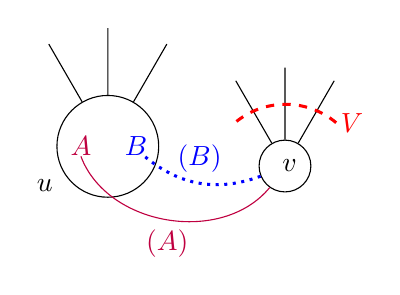
\begin{tikzpicture}
		%\draw [color=black] (0.5,-0.75) arc (-90:90:0.75);
		%\draw [color=black] (0.5,0.75) arc (90:270:0.75);
		\node [draw=none,color=purple,inner sep=0] at (0.1,0) (A) {{ $A$}};
		\node [draw=none,color=blue,inner sep=0] at (0.8,0) (B) {{ $B$}};
		\node [draw=none] at (-0.3,-.5) () {$u$};
		\node [draw,circle] at (2.75,-0.25) (v) {{ $v$}};
		\node [draw,circle,inner sep=13] at (0.5,0) (u) {};
		\draw   (u) --  +(60:1.5) (u) -- +(90:1.5) (u) -- +(120:1.5);
		\draw  (v) --  +(60:1.25) (v) -- +(90:1.25) (v) -- +(120:1.25);
		\draw [color=red,dashed,line width=1.1pt] (3.4,0.3) arc (50:130:1);
		\node [color=red] at (3.6,0.3) () {$V$};
		\draw [color=purple] (v) edge [bend left=60] node [below] {$\bbe(A)$}(A); 
		\draw [line width=1.1pt, dotted, color=blue] (v) edge [bend left=30] node [above] {$\bbe(B)$}(B); 		
	\end{tikzpicture}
	\caption{Setting of \cref{lem:<=1211good}}
	\label{fig:e(B)small}
\end{figure}

\begin{lemma}\label{lem:<=1211good}	
For a good half top edge bundle $\bbe={\bf (u,v)}$, let $A,B,C$ be the \hyperlink{tar:degreepartition}{degree partitioning} of $\delta(u)$, and  let $V=\delta(v)_{-\bbe}$ (see \cref{fig:e(B)small}). If $\eps_{1/2}\leq 0.001$, $x_{\bbe(B)}\leq \eps_{1/2}$, and $\P{(A_{-\bbe})_T + V_T\leq 1}\geq 5\eps_{1/2}$  then $\bbe$ is 2-1-1 good,
$$ \P{\bbe \text{ 2-1-1 happy w.r.t. $u$}} \geq 0.005\eps_{1/2}^2$$
\end{lemma}
\begin{proof}
The proof is similar to \cref{lem:x_e>=1/2+eps_1/2}. We condition $u,v$ to be trees, $C_T=0$, $u\cup v$  to be a tree.
Let $\nu$ be the resulting SR measure on edges in $A,B,V$.
 The main difference is since $x_\bbe\not\geq 1/2+\eps_{1/2}$ we use the lemma's assumptions to lower bound $\PP{\nu}{A_T+B_T+V_T=3},\PP{\nu}{A_T+V_T\leq 2},\PP{\nu}{B_T+V_T\leq 2}$.

%Let $\tilde{A}=A_{-\bbe}, \tilde{B}=B_{-\bbe}$.
First, since $\bbe$ is 2-2 good, by \cref{lem:2/2goodEvenSum} and negative association,
\begin{align*}
%\PP{\nu}{A_T + B_T+V_T\leq 3}&=
\PP{\nu}{(\delta(u)_{-\bbe})_T+V_T\leq 2} \geq \P{(\delta(u)_{-\bbe})_T+V_T\leq 2} - \P{C_T=0} \geq 0.4\eps_{1/2} - 2\eps_{1/1}-\eps_\eta\geq 0.22\eps_{1/2},	
\end{align*}
where we used $\eps_{1/1}\le \eps_{1/2}/12$.
Letting $p_i = \P{(\delta(u)_{-\bbe})_T+V_T = i}$, we therefore have $p_{\le 2} \ge 0.22 \eps_{1/2}$. In addition, by
\cref{thm:rayleigh_expectconstprob}, $p_3 \ge 1/4$.
%$\PP{\nu}{(\delta(u)_{-\bbe})_T+V_T=3}\geq 1/4$,   by 
If $p_2 < 0.2 \eps_{1/2}$, then from
$p_2/p_3 \le 0.8 \eps_{1/2}$, we could use log-concavity to derive a contradiction to $p_{\le 2} \ge 0.22 \eps_{1/2}$ (analogously to what's done in the proof of \cref{lem:logconcaveexpecation}).
Therefore, we must have
% (with $\gamma\leq \eps_{1/2}$) and using $\eps_{1/2}<0.001$, we have,
$$\PP{\nu}{A_T+B_T+V_T=3}=\PP{\nu}{(\delta(u)_{-\bbe})_T+V_T=2}\geq 0.2\eps_{1/2}.$$


Next, notice since $\P{u,v,u\cup v\text{ trees}, C_T=0}\geq 0.49$, by the lemma's assumption, $\PP{\nu}{\bbe(B)}\leq 2.01\eps_{1/2}$. Therefore, 
$$\EE{\nu}{B_T+V_T}\leq x(V)+x(B)+1.01\eps_{1/2}+2\eps_{1/1}+\eps_\eta \leq 2.51.$$
So, by Markov, $\PP{\nu}{B_T+V_T\leq 2}\geq 0.15$. 
%On the other hand, we claim $\EE{\nu}{B_T+V_T}\leq 1.75$. This is because conditioned on $u,v$ being trees, we choose at most 1 edge from that $\bbe$ bundle. Therefore, since under $\nu$ we choose exactly 1, the probability of choosing from $\bbe(B)$ (as opposed to $e(A)$) is at most 
%$$\frac{\EE{\nu}{e(B)_T}}{\PP{\nu}{e}} \leq \frac{x_{e(B)} + 3\eps_{1/1}}{x_{e} - 2\eps_\eta} \leq \frac{1/4-\eps_{1/2}+3\eps_{1/1}}{1/2-\eps_{1/2}-2\eps_{\eta}} \leq 1/2.$$
%Therefore, $\EE{\nu}{B_T+V_T}\leq 2.75+\eps_{1/2}+3\eps_{1/1}$. So, $\PP{\nu}{B_T+V_T\leq 2}\geq 0.08$.
Finally, by negative association, 
$$\PP{\nu}{A_T+V_T\leq 2} \geq \PP{\nu}{(A_{-\bbe})_T+V_T\leq 1} \geq \P{(A_{-\bbe})_T+V_T\leq 1} - \P{C_T=0} \geq 4.8\eps_{1/2}$$
where we used the lemma's assumption. 

Now, following the same line of arguments as in \cref{lem:x_e>=1/2+eps_1/2}, we have \\$\PP{\nu}{A_T+B_T=2 | A_T+B_T+V_T=3} \geq 0.12$.
Also, $\PP{\nu}{A_T\geq 1 | A-T+B_T+V_T=3} \geq 3.02$, which implies $\PP{\nu}{A_T=1 | A_T+B_T=2,V_T=1} \geq 0.42\eps$. This implies
$$
	\P{\bbe \text{ 2-1-1 happy}} \geq (0.42\eps_{1/2})0.12(0.2\eps_{1/2})0.498\geq 0.005\eps_{1/2}^2
$$
as desired.
\end{proof}


\lemoneoftwotwooneone*
\begin{proof}
Let $U=\delta(u)_{-\bbe}$.
By \cref{lem:crossingcorrelation}, we can assume, without loss of generality, that
\begin{equation}
\label{eq:5-26-1}
	 \E{U_T | \bbf\notin T,u,v,w\text{ tree}}\leq x(U_T)+0.405 +3\eps_{\eta}.
\end{equation}
%where we used that $\eps_{1/2}+3\eps_{\eta} < 0.001$.
On the other hand,  
\begin{align*} \E{(A_{-\bbe-\bbf})_T} &\geq \E{(A_{-\bbe-\bbf})_T|\bbf\notin T, u,v,w\text{ tree}} \P{\bbf\notin T, u,v,w,\text{ tree}}\\
&	\geq \E{(A_{-\bbe-\bbf})_T|\bbf\notin T, u,v,w\text{ tree}} 0.49
\end{align*}

So, 
\begin{equation}
\label{eq:5-26-2} 	
\E{(A_{-\bbe-\bbf})_T | \bbf\notin T, u,v,w,\text{ tree}} \leq \frac{1}{0.49} x(A_{-\bbe-\bbf}) \leq \frac{1}{0.49} (4\eps_{1/2}+\eps_{\eta}) \leq 8.2\eps_{1/2}.
\end{equation}


Combining \eqref{eq:5-26-1} and \eqref{eq:5-26-2}, we get
$\E{U_T+(A_{-\bbe}) | \bbf\notin T,u,v,w \text{ tree}}\leq 1.91$ where we used $\eps_{1/2}\leq 0.001$.
Therefore, using \cref{thm:rayleigh_expectconstprob}, we get
$$\P{U_T + (A_{-\bbe})_T\leq 1} \geq 0.49 \P{U_T + (A_{-\bbe})_T\leq 1 | \bbf\notin T,u,v,w\text{ tree}}\geq 0.01,$$
Since $\eps_{1/2}\leq 0.001$, by \cref{lem:<=1211good}, $\bbe$ is 2-1-1 good.
\end{proof}




\begin{figure*}[htb]\centering
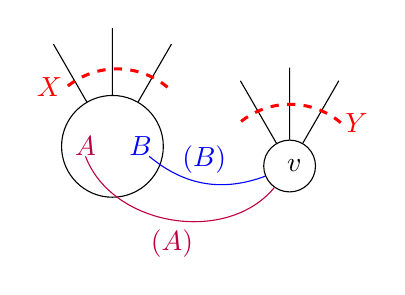
\begin{tikzpicture}
		%\draw [color=black] (0.5,-0.75) arc (-90:90:0.75);
		%\draw [color=black] (0.5,0.75) arc (90:270:0.75);
		\node [draw=none,color=purple,inner sep=0] at (0.1,0) (A) {{ $A$}};
		\node [draw=none,color=blue,inner sep=0] at (0.8,0) (B) {{ $B$}};
		%\node [draw=none] at (4,-2) () {{\Large $\hat{S}$}};
		\node [draw,circle] at (2.75,-0.25) (v) {{ $v$}};
		\node [draw,circle,inner sep=13] at (0.5,0) (u) {};
		\draw   (u) --  +(60:1.5) (u) -- +(90:1.5) (u) -- +(120:1.5);
		\draw  (v) --  +(60:1.25) (v) -- +(90:1.25) (v) -- +(120:1.25);
		\draw [color=red,dashed,line width=1.1pt] (3.4,0.3) arc (50:130:1) (1.2,0.75) arc (50:130:1);
		\node [color=red] at (3.6,0.3) () {$Y$} ;
		\node [color=red] at (-0.3,0.75) () {$X$} ;
		\draw [color=purple] (v) edge [bend left=60] node [below] {$\bbe(A)$}(A); 
		\draw [color=blue] (v) edge [bend left=30] node [above] {$\bbe(B)$}(B); 		
	\end{tikzpicture}
	\caption{Setting of \cref{lem:eABpositive211}.}
	\label{fig:e(A)e(B)large}
\end{figure*}


\lemeABpositivetwooneone*
\begin{proof}
Condition $C_T$ to be zero, $u,v$ and $u\cup v$ be trees. This happens with probability at least  $0.49$.
%Similar to the previous lemma, this doesn't happen with probability $q:=2\eps_{1/1}+3\eps_{\eta}+1/2+\eps_{1/2}$.
Let $\nu$ be the resulting measure.
Let $X=A_{-\bbe}\cup B_{-\bbe}, Y=\delta(v)_{-\bbe}$ 
Since $\bbe$ is 2-2 good by \cref{lem:2/2goodEvenSum} and stochastic dominance, 
$$\PP{\nu}{X_T + Y_T\leq 2}\geq \P{(\delta(u)_{-\bbe})_T+Y_T\leq 2} - \P{C_T=0} \geq 0.4\eps_{1/2} - 2\eps_{1/1}-\eps_\eta\geq 0.22\eps_{1/2},$$
where we used $\eps_{1/1}<12\eps_{1/2}$.
It follows by log-concavity of $X_T+Y_T$ that $\PP{\nu}{X_T+Y_T=2}\geq 0.2\eps_{1/2}$. 
Now, 
\begin{align*}
&\EE{\nu}{X_T}, \EE{\nu}{Y_T}\in [1-3\eps_{1/1}, 1.5+\eps_{1/2}+2\eps_{1/1}+3\eps_{\eta}]\subset [0.995,1.51]
\end{align*}
So,
\begin{align*}
&\PP{\nu}{X_T\geq 1}, \PP{\nu}{Y_T\geq 1}\geq 0.63, \tag{\cref{lem:SR>=}} \\
&\PP{\nu}{X_T\leq 1}, \PP{\nu}{Y_T\leq 1}\geq 0.245.\tag{Markov}
\end{align*}
Therefore, by \cref{lem:SRA=nA} $\PP{\nu}{X_T= 1 | X_T+Y_T=2}\geq 0.119$.
$$ \PP{\nu}{X_T=Y_T=1} \geq (0.2\eps_{1/2}) 0.119 \geq 0.023\eps_{1/2},$$
Let $\cE$ be the event $\{X_T=Y_T=1 | \nu\}$.
Note that in $\nu$ we always choose exactly 1 edge from the $\bbe$ bundle and that is independent of edges in $X,Y$, in particular the above event. Therefore, we can  correct the parity of $A,B$ by choosing from $e_A$ or $e_B$.
It follows that
$$ \P{\bbe \text{ 2-1-1 happy w.r.t $u$}} \geq \PP{\nu}{\cE}(1.99\eps_{1/2}) 0.49 \geq 0.02\eps_{1/2}^2,$$
where we used that $\EE{\nu}{\bbe(A)_T}  \geq 1.99\eps_{1/2}$, and the same fact for $\bbe(B)_T$. To see why this latter fact is true, observe that conditioned on $u,v$ trees, we always sample at most one edge between $u,v$. Therefore, since under $\nu$ we choose exactly one edge between $u,v$, the probability of choosing from $e(A)$ (and similarly choosing from $\bbe(B)$) is at least 
$$\frac{\E{\bbe(A)_T | u,v\text{ trees}, C_T=0}}{\P{\bbe | u,v\text{ trees}, C_T=0}} \geq \frac{x_{\bbe(A)}-2\eps_\eta}{x_{\bbe}+3\eps_{1/1}}\geq \frac{\eps_{1/2}-2\eps_{\eta}}{1/2+1.3\eps_{1/2}}\geq 1.99\eps_{1/2}$$
as desired.
\end{proof}




\begin{figure}[htb]\centering
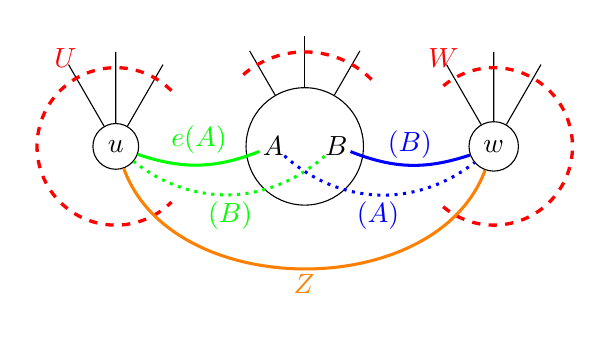
\begin{tikzpicture}[scale=0.8]
\tikzstyle{every node}=[draw,circle]
\foreach \a/\x/\l in {u/-3/U, w/3/W}{
\path  (\x,0) node  (\a) {$\a$};
\path (\a)+(-0.8,1.4) node [color=red,draw=none] (){$\l$};
\foreach \xx in {0,...,2}{
\draw [-] (\a) -- ++(60+\xx*30: 1.5);}
}
\draw [dashed,color=red,line width=1.2] (u)+(45:1.25) arc (45:315:1.25);
\draw [dashed,color=red,line width=1.2] (w)+(-130:1.25) arc (-130:130:1.25);


\node [inner sep=15] at (0,0) (v) {};
\foreach \xx in {0,...,2}{
\draw [-] (v) -- ++(60+\xx*30: 1.75);}
\draw [dashed,color=red,line width=1.2] (v)+(45:1.5) arc (45:135:1.5);

\node [draw=none,inner sep=0] at (-.5,0) (A) {$A$};
\node [draw=none,inner sep=0] at (.5,0) (B) {$B$};

\path [-] (A) edge [bend left=20,color=green,line width=1.1pt] node [draw=none,above=-7pt] {$e(A)$} (u)
(B) edge [bend left=40,color=green, line width=1.1pt,dotted] node [draw=none,below=-7pt] {$\bbe(B)$} (u)
(A) edge [bend right=40,color=blue, line width=1.1pt, dotted] node [draw=none, below=-7pt] {$\bbf(A)$} (w)
(B) edge [bend right=20,color=blue, line width=1.1pt] node [draw=none,above=-7pt] {$\bbf(B)$} (w)
;
\path (u) edge [color=orange,bend right=70,line width=1.1pt] node [draw=none,below=-5pt] {$Z$} (w);
\end{tikzpicture}
\caption{Setting of \cref{lem:222}. We assume that the dotted green/blue edges are at most $\eps_{1/2}$. Note that edges of $C$ are not shown.} 
\label{fig:eABpositive211}
\end{figure}
\lemtwotwotwo*
\begin{proof}
%	Let $e(A)=e\cap A$ and $e(B),f(A),f(B)$ are similarly defined.
%	First, by \cref{lem:eABpositive211} if $x_{e(A)},x_{e(B)}\geq \eps_{1/2}$, then $\bbe$ is 2-1/1 good (w.r.t., $v$).
%	Similarly, we will be done if $x_{f(A)},x_{f(B)}\geq  \eps_{1/2}$. Furthermore by \cref{lem:one-of-two-211} if $x_{e(B)},x_{f(B)}\leq \eps_{1/2}$ then one of $e,f$ is 2-1/1 good.
%	The only remaining case is when $x_{e(B)},x_{f(A)}<\eps_{1/2}$.
	%	Without loss of generality let $e'=A\cap\delta(u)$.
%	
	First, observe that by \cref{lem:<=1211good} if $\P{U_T+(A_{-\bbe})_T\leq 1}\geq 0.25\eps$, where $\eps\geq 20\eps_{1/2}$ is a constant that we fix later, then $\bbe$ is 2-1-1 good, which is a contradiction. 
	So, assume, $\P{U_T+(A_{-\bbe})_T\geq 2}\geq 1-0.25\eps.$
	Furthermore, let $q=\P{U_T+(A_{-\bbe})_T\geq 3}$. Since $x(U)+x(A_{-\bbe})\leq 2+3\eps_{1/2}+2\eps_{1/1}+3\eps_\eta\leq 2+3.2\eps_{1/2}$ (where we used $x_{\bbe(A)}\geq x_\bbe - x_{\bbe(B)} - x_C\geq  1/2-2\eps_{1/2}-2\eps_{1/1}-\eps_{\eta}$ and where we used $12\eps_{1/1}\leq \eps_{1/2}$), 
	$$ 2(1-q-0.25\eps) +3q \leq 2+3.2\eps_{1/2}.$$
	This implies that $q\leq 0.5\eps + 3.2\eps_{1/2}\leq 0.75\eps$ (for $\eps\geq  13\eps_{1/2})$.
	Therefore, 
%	Similarly, if $\P{W_T+(B_{-\bbf})_T\leq 1}\geq \eps/4$, then $f$ is 2-1/1 good and we are done.
	\begin{equation}\label{eq:211-bad}
		\P{U_T+(A_{-\bbe})_T=2},\P{W_T+(B_{-\bbf})_T=2}\geq 1-\eps
	\end{equation}
	where the second inequality follows by a similar argument.
	\begin{claim} 	Let $Z=\delta(u)\cap\delta(w)$. If $\eps<1/15$, then either
		$\E{Z | u,v,w\text{ tree}}\leq 3\eps$ or $\E{Z | u,v,w\text{ tree}}\geq (1-3\eps)$.
	\end{claim}
\begin{proof}
For the whole proof we work with $\mu$ conditioned on $u,v,w$ are trees.
	Let $z=\E{Z}$.
	Let $D=U\cup W\cup A_{-\bbe}\cup B_{-\bbf}\smallsetminus Z$. Note that $D_T+2Z_T=U_T\cup W_T\cup (A_{-\bbe})_T\cup (B_{-\bbf})_T$.
	By \cref{eq:211-bad} and a union bound $\P{D_T+2Z_T=4}\geq 1-2\eps-3\eps_\eta$. Therefore,
	\begin{align*}
		2.1\eps\geq 2\eps+3\eps_\eta  \geq \P{D_T+2Z_T\neq 4} \geq \P{D_T=3} \geq \sqrt{\P{D_T=2}\P{D_T=4}}
	\end{align*}
	where the last inequality follows by log-concavity.
%	In the rest of the proof we use $3\eps_\eta < 0.1\eps$.
	On the other hand,  
	\begin{align*} &z=\P{Z=1} \leq \P{D_T=2,Z=1}+\P{D_T+2Z_T\neq 4} \leq \P{D_T=2} + 2.1\eps,\\	
&	1-z=\P{Z=0} \leq \P{D_T=4,Z=0}+\P{D_T+2Z_T\neq 4} \leq \P{D_T=4} + 2.1 \eps
	\end{align*}
%	and similarly, $\P{D_T=4}\geq 1-z-2.1\eps$. 
Putting everything together,
	$$(2.1\eps)^2 \geq (z-2.1\eps)(1-z-2.1\eps)=z(1-z)-2.1\eps + 2.1\eps^2.$$
	Therefore, using $\eps\leq 1/15$, we get that either $z\leq 3\eps$ or $z\geq 1-3\eps$.
\end{proof}
%So, for the rest of proof we assume $\E{Z_T|u,v,w \text{ trees}}<3\eps$. A similar proof shows $\bbe,\bbf$ are 2-2-2 good when  $\E{Z_T|u,v,w\text{ trees}}>1-3\eps$.
%We run the following conditionings in order: $u,v,w$ trees, $Z_T=0$, $C_T=0$, $\bbe(B),\bbf\notin T$, $\bbe(A)\in T$. Note that $\bbe(A)\in T$ is equivalent to $u\cup v$ be a tree. Call this event $\cE$ (i.e., the event that all 8 things we conditioned on happen).
%First, notice 
%$$\P{\cE}\geq (1-3\eps_\eta) (1-3\eps-2\eps_{1/1}-\eps_\eta-\eps_{1/2}-(1/2+\eps_{1/2}))  (1/2-3\eps_{1/2})\geq 0.22\geq 1/5$$
%Note that all of these conditionings correspond to upward/downward events, so $\mu | \cE$ is strongly Rayleigh.
%The main statement we need to show is that $\P{U_T=(A_{-\bbe})_T=1, (B_{-\bbf})_T=0,W_T=2|\cE}\geq \Omega(1)$. The main insight of the proof is that \cref{eq:211-bad} holds (up to a larger constant of $\eps$), even after conditioning $\cE, B_{-\bbf}=0,A_{-\bbe}=1$; so, we can bound the preceding event by just a union bound. The main non-trivial statement is to argue that the expectations of $B_{-\bbf}$ and $A_{-\bbe}$ do not change so much under $\cE$.
%
%By a union bound and \eqref{eq:211-bad}
%\begin{equation}\label{eq:211-badcE} \P{U_T+(A_{-\bbe})_T=2 | \cE},\P{W_T+(B_{-\bbf})_T=2 | \cE}\geq 1-5\eps.	
%\end{equation}
%We claim that 
%$$\E{B_T | \cE}=\E{(B_{-\bbf})_T|\cE} \leq x(B_{-\bbf}) + 3\eps+ 3\eps_{1/1}+ \eps_{1/2} +30 \eps \leq 0.64,$$
%using $\eps_{1/2}<0.0005$ and $\eps= 20\eps_{1/2}$.
%%$(B_{-\bbf})_T=0$. 
%To see this, observe that after each conditioning in $\cE$ either all marginals increase or all decrease. Furthermore, the events $C_T=0, Z_T=0, e(A)_T=0$ can increase marginals by at most $3\eps+3\eps_{1/1}+\eps_{1/2}$; the only other event that can increase $B_{-\bbf}$ is $\bbf\notin T$. Now, suppose under $\bbf\notin T$, $\E{(B_{-\bbf})_T}$ increases by more than $30\eps$. Since this event does not decrease $W_T$, this means that either before conditioning $\bbf\notin T$,  $\E{(B_{-\bbf})+W_T}<2-10\eps$ or afterwards it is more than $2+20\eps$. But, by \cref{cor:logconcaveexpecation} the former is in contradiction with $\P{(B_{-\bbf})+W_T=2 | u,v,w\text{ tree}, Z_T=C_T=0,\bbe(B)\notin T}\geq 1-5\eps$,  and the latter with \cref{eq:211-badcE}.
%Similarly, $\E{(A_{-\bbe})_T|\cE}\leq 0.64$.
%
%%: Since 
%%\begin{align*}\E{(B_{-\bbf})_T+W_T | u,v,w\text{ trees}, Z_T=C_T=0,e(B)\notin T}&\geq \E{(B_{-\bbf})_T+W_T} -3\eps_{\eta}\\
%%&\geq 2-4\eps_{1/2}\geq 2-\eps.
%%\end{align*}
%%%\E{(B_{-\bbf})_T+W_T | u,v,w\text{ trees}, Z_T=C_T=0,e(B)\notin T}\geq 2-10\eps$. 
%%On the other hand, since $\P{(B_{-\bbf})_T+W_T=3 | \cE}\leq 5\eps$, by \cref{lem:logconcaveexpecation} with $\gamma=6\eps$, 
%%$$\P{(B_{-\bbf})_T+W_T\geq 3| \cE}\E{(B_{-\bbf})_T+W_T | (B_{-\bbf})_T+W_T\geq 3, \cE}\leq \frac{5\eps}{1-6\eps}(3+7\eps)\leq 17\eps$$
%%so, $\E{(B_{-\bbf})_T+W_T|\cE}\leq 2+7\eps$.
%We claim,
%$$\E{(A_{-e})_T | \cE} \geq x(A_{-e}) - 3\eps_{\eta} -35\eps$$
%We know $\P{U_T+(A_{-e})_T=2 |\cE}\geq 1-5\eps$ before and after $\bbe(A)\notin T$. By Corollary 2.19, $2-10\eps \leq \E{U_T+(A_{-e})_T}\leq 2+10\eps+15\eps$. 
%
%Following a similar argument $\E{(A_{-\bbe})_T | \cE}\geq x(A_{-\bbe}) -40\eps \geq 0.33$.
%
%It follows that
%$$ 0.33\leq \E{(A_{-\bbe})_T |\cE}\leq \E{(A_{-\bbe})_T | \cE,(B_{-\bbf})_T=0} \leq 0.64 +0.64\leq 1.28.  $$
%So, by \cref{thm:rayleigh_expectconstprob} and \cref{thm:hoeffding}, $\P{(A_{-\bbe})_T=1 | \cE, (B_{-f})_T=0}\geq 0.33e^{-.33}\geq 0.237$.
%
%%e^(-1.28)*1.28*(1-1.28/2)^0.28 (l=0)
%
%Therefore, by \cref{thm:rayleigh_expectconstprob}
%$$ \P{\cE,(A_{-\bbe})_T=1,(B_{-\bbf})_T=0} \geq (0.22)(0.39)(0.23)\geq  0.019.$$
%Therefore, by union bound and \eqref{eq:211-badcE}
%$$ \P{U_T=1 | \cE,(A_{-\bbe})_T=1,(B_{-\bbf})_T=0}, \P{W_T=2 | \cE,(A_{-\bbe})_T=1,(B_{-\bbf})_T=0}\geq 1-\eps/0.019$$
%Finally, by union bound 
%$$ \P{U_T=1, W_T=2 | \cE,(A_{-\bbe})_T=1,(B_{-\bbf})_T=0}\geq 1-\eps/0.009$$
%Using $\eps=20\eps_{1/2}$ and $\eps_{1/2}\leq 0.0002$ this means both of the above event happens, so that $\bbe,\bbf$ are 2-2-2 happens with probability $0.019(1-\eps/0.009) > 0.01$ as desired.
%
%
%\vspace{1in}

%%%%%%%%%%%%%%%%%%%%%%%%%%%%%%%

So, for the rest of proof we assume $\E{Z_T|u,v,w \text{ trees}}<3\eps$. A similar proof shows $\bbe,\bbf$ are 2-2-2 good when  $\E{Z_T|u,v,w\text{ trees}}>1-3\eps$.
We run the following conditionings in order: $u,v,w$ trees, $Z_T=0$, $C_T=0$, $\bbe(B),\bbf\notin T$, $\bbe(A)\in T$. Note that $\bbe(A)\in T$ is equivalent to $u\cup v$ be a tree. Call this event $\cE$ (i.e., the event that all things we conditioned on happen).
First, notice 
\begin{equation}
\label{eq:cElb}\P{\cE}\geq (1-3\eps_\eta) (1-3\eps-2\eps_{1/1}-\eps_\eta-\eps_{1/2}-(1/2+\eps_{1/2}))  (1/2-3\eps_{1/2})\geq 0.22\geq 1/5
\end{equation}	


Moreover, since all of these conditionings correspond to upward/downward events,  $\mu | \cE$ is strongly Rayleigh.
The main statement we will show is that $$\P{\bbe,\bbf\text{ 2-2-2 happy}|\cE}\ge \P{U_T=(A_{-\bbe})_T=1, (B_{-\bbf})_T=0,W_T=2|\cE}= \Omega(1).$$
The main insight of the proof is that \cref{eq:211-bad} holds (up to a larger constant of $\eps$), even after conditioning $\cE, B_{-\bbf}=0,A_{-\bbe}=1$; so, we can bound the preceding event by just a union bound. The main non-trivial statement is to argue that the expectations of $B_{-\bbf}$ and $A_{-\bbe}$ do not change so much under $\cE$.

Combining \eqref{eq:211-bad} and \eqref{eq:cElb},
\begin{equation}\label{eq:211-badcE} \P{U_T+(A_{-\bbe})_T=2 | \cE},\P{W_T+(B_{-\bbf})_T=2 | \cE}\geq 1-5\eps.	
\end{equation}
We claim that 
\begin{equation}
\label{eq:BTcondcE}
	\E{B_T | \cE}=\E{(B_{-\bbf})_T|\cE} \leq x(B_{-\bbf}) + 3\eps_\eta+ 3\eps_{1/1}+ \eps_{1/2} +35 \eps \leq 0.66 %\text{ 
%\anna{(old $30 \eps$, got 0.66)}},
\end{equation}
using $\eps_{1/2}<0.0002$ and $\eps= 20\eps_{1/2}$.
%$(B_{-\bbf})_T=0$. 
To see this, observe that after each conditioning in $\cE$ either all marginals increase or all decrease. Furthermore, the events $C_T=0, Z_T=0, \bbe(B)_T=0$ can increase marginals by at most $3\eps_\eta+3\eps_{1/1}+\eps_{1/2}$; the only other event that can increase $B_{-\bbf}$ is $\bbf\notin T$. Now 
we know $\P{(B_{-\bbf})_T+W_T=2 |\cE}\geq 1-5\eps$ before and after conditioning $\bbf\notin T$. Therefore, by Corollary 2.19, $2-10\eps \leq \E{(B_{-\bbf})_T+W_T}\leq 2+25\eps$. 
But if $\E{(B_{-\bbf})_T}$ increased by more than $35\eps$, then either before conditioning $\bbf\notin T$,  $\E{(B_{-\bbf})+W_T}<2-10\eps$ or afterwards it is more than $2+25\eps$, which is a contradiction, and completes the proof of \eqref{eq:BTcondcE}.
A similar argument shows that $\E{(A_{-\bbe})_T|\cE}\leq 0.66$.

%: Since 
%\begin{align*}\E{(B_{-\bbf})_T+W_T | u,v,w\text{ trees}, Z_T=C_T=0,e(B)\notin T}&\geq \E{(B_{-\bbf})_T+W_T} -3\eps_{\eta}\\
%&\geq 2-4\eps_{1/2}\geq 2-\eps.
%\end{align*}
%%\E{(B_{-\bbf})_T+W_T | u,v,w\text{ trees}, Z_T=C_T=0,e(B)\notin T}\geq 2-10\eps$. 
%On the other hand, since $\P{(B_{-\bbf})_T+W_T=3 | \cE}\leq 5\eps$, by \cref{lem:logconcaveexpecation} with $\gamma=6\eps$, 
%$$\P{(B_{-\bbf})_T+W_T\geq 3| \cE}\E{(B_{-\bbf})_T+W_T | (B_{-\bbf})_T+W_T\geq 3, \cE}\leq \frac{5\eps}{1-6\eps}(3+7\eps)\leq 17\eps$$
%so, $\E{(B_{-\bbf})_T+W_T|\cE}\leq 2+7\eps$.
We also claim that
$$\E{(A_{-e})_T | \cE} \geq x(A_{-e}) - 3\eps_{\eta} -35\eps \ge 0.33.$$
As above, everything conditioned on in $\cE$ increases $\E{(A_{-e})_T }$ except for possibly $\bbe(A)\in T$.  As above, we know that $\P{U_T+(A_{-e})_T=2 |\cE}\geq 1-5\eps$ before and after $\bbe(A)\notin T$. So again applying Corollary 2.19, we see that it can't decrease by more than $35 \eps$.


It follows that
$$ 0.33\leq \E{(A_{-\bbe})_T |\cE}\leq \E{(A_{-\bbe})_T | \cE,(B_{-\bbf})_T=0} \leq 0.66 +0.66\leq 1.32.  $$
So, by \cref{thm:rayleigh_expectconstprob} and \cref{thm:hoeffding}, $\P{(A_{-\bbe})_T=1 | \cE, (B_{-f})_T=0}\geq 0.33e^{-.33}\geq 0.237$.

%e^(-1.28)*1.28*(1-1.28/2)^0.28 (l=0)

Therefore, by \cref{thm:rayleigh_expectconstprob}
$$ \P{\cE,(A_{-\bbe})_T=1,(B_{-\bbf})_T=0} \geq (0.22)(0.39)(0.23)\geq  0.019.$$
Therefore, by  \eqref{eq:211-badcE}
$$ \P{U_T=1 | \cE,(A_{-\bbe})_T=1,(B_{-\bbf})_T=0}, \P{W_T=2 | \cE,(A_{-\bbe})_T=1,(B_{-\bbf})_T=0}\geq 1-5\eps/0.019$$
Finally, by union bound 
$$ \P{U_T=1, W_T=2 | \cE,(A_{-\bbe})_T=1,(B_{-\bbf})_T=0}\geq 1-\eps/0.009$$
Using $\eps=20\eps_{1/2}$ and $\eps_{1/2}\leq 0.0002$ this means both of the above events happens, so  $\bbe,\bbf$ are 2-2-2-happy with probability $0.019(1-\eps/0.009) > 0.01$ as desired.
\end{proof}
